\documentclass{article}

\usepackage[main, final]{neurips_2025}

\usepackage[utf8]{inputenc}
\usepackage[T1]{fontenc}
\usepackage{hyperref}
\usepackage{url}
\usepackage{booktabs}
\usepackage{amsmath}
\usepackage{amsfonts}
\usepackage{amssymb}
\usepackage{amsthm}
\usepackage{nicefrac}
\usepackage{microtype}
\usepackage{xcolor}
\usepackage{graphicx}
\usepackage{multirow}
\usepackage{multicol}
\usepackage{float}

\newtheorem{definition}{Definition}

% Pack text more tightly around floats (default style traps whitespace
% on figure-heavy pages).
\renewcommand{\topfraction}{0.95}
\renewcommand{\textfraction}{0.05}
\renewcommand{\floatpagefraction}{0.85}
\setcounter{topnumber}{3}
\setcounter{totalnumber}{4}

\newcommand{\Elog}{S_{\mathrm{log}}}
\newcommand{\Equad}{S_{\mathrm{quad}}}
\newcommand{\Eenergy}{S_{\mathrm{E}}}
\newcommand{\Ekernel}{S_{\mathrm{K}}}
\newcommand{\simplex}{\Delta^{V-1}}

\title{Beyond Perplexity: Evaluating LLM Token Distributions\\with Proper Scoring Rules}

\author{%
  Zhicheng You \\
  \And
  Sagarima Datta \\
}

\begin{document}

\maketitle

\begin{abstract}
  The evaluation of language models is dominated by perplexity, the exponentiated mean
  log-score, which assesses predictive distributions exclusively through the Bregman
  geometry of the Kullback--Leibler divergence. We evaluate three open autoregressive
  language models (GPT-2, GPT-2-Medium, OPT-125M) on WikiText-103 and the Penn Treebank
  under four strictly proper scoring rules---the log-score, the quadratic (Brier) score,
  the energy score, and the Gaussian-kernel (MMD) score---each of which, by the Savage
  representation, evaluates forecasts through the Bregman divergence of a distinct convex
  generator. Across 20{,}000 scored token positions per model--corpus pair we report four
  findings. First, the rules do not rank the models identically: the energy score prefers
  OPT-125M while the remaining rules unanimously prefer GPT-2-Medium, and a nonparametric
  bootstrap reproduces this disagreement in every resample. Second, the penalty each rule
  assigns to rare tokens scales with the boundary curvature of its generator: from the
  most- to the least-frequent decile the log-score grows $2.05\times$, against
  $1.22\times$ for the bounded quadratic score. Third, the log-to-energy penalty ratio
  widens by $47\%$ from low- to high-entropy predictions, as the locality of the
  Kullback--Leibler divergence predicts. Fourth, a centroid analysis of more than
  $13{,}000$ misprediction events shows that the energy ranking tracks the distance
  between the predictive barycenter and the realized token in embedding space---the
  quantity the energy divergence is constructed to measure. Together, the experiments
  constitute an empirical verification of the Bregman account of scoring-rule
  disagreement and motivate reporting complementary proper scoring rules alongside
  perplexity. Code: \url{https://github.com/sagarima-datta/beyond-perplexity}.
\end{abstract}

\section{Introduction}

At every generation step an autoregressive language model produces a complete probability
distribution over its vocabulary. The prevailing evaluation practice reduces this object
to a single statistic, perplexity, computed from the log-score $-\log p(y)$ of the
realized token $y$. The choice is historically motivated \citep{jelinek1977} rather than
derived from first principles: the log-score is one member of the family of
\emph{strictly proper scoring rules} \citep{gneiting2007}, and each member of that
family evaluates forecasts through a different divergence geometry. Reliance on
perplexity alone therefore amounts to an implicit assumption that the Kullback--Leibler
(KL) geometry is appropriate for all model comparisons. The present work examines that
assumption empirically.

We score three publicly available causal language models under four strictly proper
scoring rules on two corpora, asking three questions. \textbf{(Q1)} Do the rules induce
the same model ranking? \textbf{(Q2)} Where they disagree, is the disagreement
statistically robust, and is it predicted by the geometry of the rules' Bregman
generators? \textbf{(Q3)} Can the mechanism of a disagreement be located in the
structure of the predictive distributions themselves?

\paragraph{Contributions.} The paper makes three contributions.
\begin{enumerate}
  \item A systematic comparison of four strictly proper scoring rules (log, quadratic,
        energy, kernel) over $3$ models $\times$ $2$ corpora $\times$ $20{,}000$ token
        positions, with per-token score caches permitting token-level concordance
        analysis (Sections~\ref{sec:exp1}--\ref{sec:exp3}).
  \item A bootstrap certification that the observed inter-rule ranking disagreement is
        not attributable to sampling variability (Section~\ref{sec:exp4}).
  \item An experiment-by-experiment verification that the observed score behavior is
        the behavior the Savage--Bregman representation requires: tail penalties order
        with generator curvature (Section~\ref{sec:exp2}), uncertainty penalties with
        locality (Section~\ref{sec:exp3}), and the energy ranking coincides with the
        ordering of predictive-barycenter distances in embedding space
        (Section~\ref{sec:exp5}).
\end{enumerate}

\section{Theoretical background}
\label{sec:theory}

\subsection{Proper scoring rules}

Let $\mathcal{V} = \{1,\dots,V\}$ denote the vocabulary and $\simplex$ the probability
simplex over $\mathcal{V}$. A (negatively oriented) scoring rule is a function
$S : \simplex \times \mathcal{V} \to \mathbb{R}$ assigning loss $S(P,y)$ to the forecast
$P$ upon realization of $y$. Writing $S(P,Q) = \mathbb{E}_{y\sim Q}\, S(P,y)$ for the
expected loss under data distribution $Q$, the rule is \emph{proper} if
$S(Q,Q) \le S(P,Q)$ for all $P, Q \in \simplex$, and \emph{strictly proper} if equality
implies $P = Q$. Strict properness is the minimal requirement for honest evaluation: it
renders truthful reporting of beliefs the unique minimizer of expected loss.

\subsection{The Bregman representation theorem}
\label{sec:bregman}

The structural result on which our analysis rests is the Savage representation
\citep{gneiting2007}: a regular scoring rule $S$ is (strictly) proper if and only if
there exists a (strictly) convex function $\varphi : \simplex \to \mathbb{R}$---the
negative generalized entropy of the rule, recoverable as $\varphi(P) = -S(P,P)$---such
that
\begin{equation}
  S(P, y) \;=\; -\varphi(P) \;-\; \big\langle \nabla\varphi(P),\, e_y - P \big\rangle ,
  \label{eq:savage}
\end{equation}
where $e_y$ denotes the vertex of the simplex at $y$. The score of an outcome is thus the
negated evaluation, at $e_y$, of the supporting hyperplane of $\varphi$ drawn at the
forecast. Taking expectations of Equation~\eqref{eq:savage} under $y \sim Q$ and
subtracting the oracle score yields the divergence form
\begin{equation}
  S(P, Q) - S(Q, Q) \;=\; d_\varphi(Q, P)
  \;:=\; \varphi(Q) - \varphi(P) - \langle \nabla\varphi(P),\, Q - P\rangle ,
  \label{eq:bregman}
\end{equation}
the Bregman divergence generated by $\varphi$, i.e., the gap between $\varphi$ at $Q$ and
the tangent of $\varphi$ constructed at $P$. Three consequences of
Equation~\eqref{eq:bregman} organize the experiments that follow.

First, \emph{properness is convexity}. The expected regret on the left of
Equation~\eqref{eq:bregman} is nonnegative precisely because a convex function dominates
its tangents, and vanishes uniquely at $P = Q$ precisely when $\varphi$ is strictly
convex; the properness of a rule is constituted by its geometry.

Second, \emph{each rule is a choice of geometry}. The generator $\varphi$ endows the
simplex with a curvature, and $d_\varphi$ measures forecast error along it. By
Equation~\eqref{eq:bregman}, ``model $A$ outperforms model $B$ under rule $S$'' is
the statement that $A$'s predictive distributions lie closer
to the data distribution in the geometry of $\varphi_S$. Table~\ref{tab:generators}
records the generators and divergences of the four rules evaluated here. The curvature of
the log-score's generator, $\nabla^2\varphi = \operatorname{diag}(1/p_v)$, diverges at
the boundary of the simplex; the quadratic generator has constant Hessian $2I$; the
energy and kernel generators inherit their curvature from the metric structure of an
embedding space and are consequently the only rules in the suite for which the notion of
\emph{similarity between tokens} is defined. These curvature properties yield concrete,
falsifiable predictions about score behavior---predictions the experiments below test.

Third, \emph{inter-rule disagreement is informative}. If two strictly proper rules rank
models differently, Equation~\eqref{eq:bregman} implies the models' distributions stand
at different relative distances from the data distribution under two distinct
curvatures. Throughout Sections~\ref{sec:exp1}--\ref{sec:exp5} we accordingly treat each
disagreement as a measurement to be explained, asking in each case whether the observed
pattern is the one the relevant generators require.

\begin{table}[t]
  \caption{Savage--Bregman generators of the four evaluated rules. Here
  $X, X' \stackrel{\text{iid}}{\sim} P$, $e(\cdot)$ denotes the embedding map, and $k$ is
  the Gaussian kernel. Each generator is recovered as $\varphi(P) = -S(P,P)$; strict
  convexity of $\varphi$ is equivalent to strict properness of the rule.}
  \label{tab:generators}
  \centering
  \small
  \begin{tabular}{lll}
    \toprule
    Rule & Generator $\varphi(P)$ & Divergence $d_\varphi$ \\
    \midrule
    Log        & $\sum_v p_v \log p_v$ \ (negative Shannon entropy) & Kullback--Leibler \\
    Quadratic  & $\lVert p \rVert_2^2 - 1$ & squared Euclidean on $\simplex$ \\
    Energy     & $-\tfrac{1}{2}\,\mathbb{E}\lVert e(X) - e(X')\rVert$ & energy distance (via $e$) \\
    Kernel     & $\mathbb{E}\,k\big(e(X), e(X')\big) - 1$ & squared MMD (via $e$, $k$) \\
    \bottomrule
  \end{tabular}
\end{table}

\subsection{The four rules}
\label{sec:rules}

All rules below are strictly proper and negatively oriented (lower is better). We write
$p_v$ for the forecast probability of token $v$ and $X, X' \stackrel{\text{iid}}{\sim} P$.

\paragraph{Log-score.} $\Elog(P,y) = -\log p_y$, with KL divergence as its Bregman
divergence. The rule is \emph{local}---it depends on $P$ only through the coordinate
$p_y$, and is in fact the only smooth, local, strictly proper rule---but locality
entails that the score is unbounded and insensitive to the placement of the remaining
$1 - p_y$ probability mass.

\paragraph{Quadratic (Brier) score.} $\Equad(P,y) = \lVert p - e_y\rVert_2^2$, with
squared Euclidean distance as its divergence. The rule is bounded on $[0,2]$ and global:
mass misplaced anywhere on the simplex is penalized, though no metric structure on the
vocabulary enters.

\paragraph{Energy score.} Given a feature map $v \mapsto e(v) \in \mathbb{R}^d$---here,
each model's input-embedding matrix $E \in \mathbb{R}^{V\times d}$---the energy score
\citep{gneiting2007,szekely2013} is
\begin{equation}
  \Eenergy(P,y) \;=\; \mathbb{E}\,\lVert e(X)-e(y)\rVert
  \;-\; \tfrac{1}{2}\,\mathbb{E}\,\lVert e(X)-e(X')\rVert .
  \label{eq:energy}
\end{equation}
Its divergence is the energy distance between $P$ and the point mass $\delta_y$,
computed through $e(\cdot)$. The rule is distance-sensitive: errors concentrated in the
embedding neighborhood of the target are penalized less than errors of equal probability
dispersed far from it.

\paragraph{Kernel (MMD) score.} For the Gaussian kernel
$k(x,x') = \exp\!\big(-\lVert x-x'\rVert^2 / 2\sigma^2\big)$,
\begin{equation}
  \Ekernel(P,y) \;=\; k\big(e(y),e(y)\big) - 2\,\mathbb{E}\,k\big(e(X), e(y)\big)
  + \mathbb{E}\,k\big(e(X), e(X')\big),
  \label{eq:kernel}
\end{equation}
the squared maximum mean discrepancy between $P$ and $\delta_y$ in the reproducing-kernel
Hilbert space of $k$ \citep{gretton2012,steinwart2021}. The exponential decay of the
kernel beyond its bandwidth $\sigma$ gives the rule a locality window: mass at distances
much greater than $\sigma$ from the target contributes to the score only through the
self-similarity term. We set $\sigma$ per model by the median heuristic (the median
pairwise distance between vocabulary embeddings), the standard choice in the MMD
literature.

\section{Experimental setup}
\label{sec:setup}

\paragraph{Models.} GPT-2 (117M parameters), GPT-2-Medium (345M)
\citep{radford2019}, and OPT-125M \citep{zhang2022}, obtained from the Hugging Face Hub
and evaluated in single precision on CPU. The GPT-2 variants share a byte-level BPE
tokenizer (50{,}257 types); OPT employs a closely related vocabulary (50{,}265 types).

\paragraph{Corpora.} The WikiText-103 test split (encyclopedic prose) and the Penn
Treebank as distributed through NLTK (newswire). Documents are tokenized with each
model's own tokenizer, truncated to 512 tokens, and scored autoregressively until
20{,}000 positions are accumulated per (model, corpus) cell.

\paragraph{Estimation.} The log and quadratic scores are computed in closed form from the
softmax vector. The energy and kernel scores are estimated by paired Monte Carlo
sampling: at each position two independent samples of size $m = 200$ are drawn from $P$
and substituted into the unbiased plug-in forms of Equations~\eqref{eq:energy}
and~\eqref{eq:kernel} (Appendix~\ref{app:impl}). Kernel bandwidths obtained by the median
heuristic are $\sigma_0 = 4.82$ (GPT-2), $4.37$ (GPT-2-Medium), and $1.97$ (OPT-125M).
Per-token scores for every cell are cached, so all downstream analyses operate on
identical score arrays.

\section{Experiment 1: global rankings under the four rules}
\label{sec:exp1}

\begin{table}[t]
  \caption{Mean scores over 20{,}000 token positions (lower is better). Boldface marks
  the best model under each rule and corpus.}
  \label{tab:exp1}
  \centering
  \small
  \begin{tabular}{llcccc}
    \toprule
    Corpus & Model & Log & Quadratic & Energy & Kernel \\
    \midrule
    \multirow{3}{*}{WikiText-103}
      & GPT-2        & 3.917 & 0.807 & 1.466 & 0.205 \\
      & GPT-2-Medium & \textbf{3.591} & \textbf{0.774} & 1.223 & \textbf{0.183} \\
      & OPT-125M     & 4.049 & 0.811 & \textbf{0.812} & 0.327 \\
    \midrule
    \multirow{3}{*}{PTB}
      & GPT-2        & 5.028 & 0.892 & 1.646 & 0.231 \\
      & GPT-2-Medium & \textbf{4.769} & \textbf{0.875} & 1.394 & \textbf{0.208} \\
      & OPT-125M     & 5.199 & 0.907 & \textbf{0.935} & 0.382 \\
    \bottomrule
  \end{tabular}
\end{table}

Table~\ref{tab:exp1} reports the principal comparison. Under the log, quadratic, and
kernel scores the verdict is unanimous on both corpora:
GPT-2-Medium $\succ$ GPT-2 $\succ$ OPT-125M. The energy score alone inverts this
ordering, ranking OPT-125M first by a substantial margin (0.812 against 1.223 on
WikiText-103) while the same model is ranked last by every other rule.

\begin{figure}[t]
  \centering
  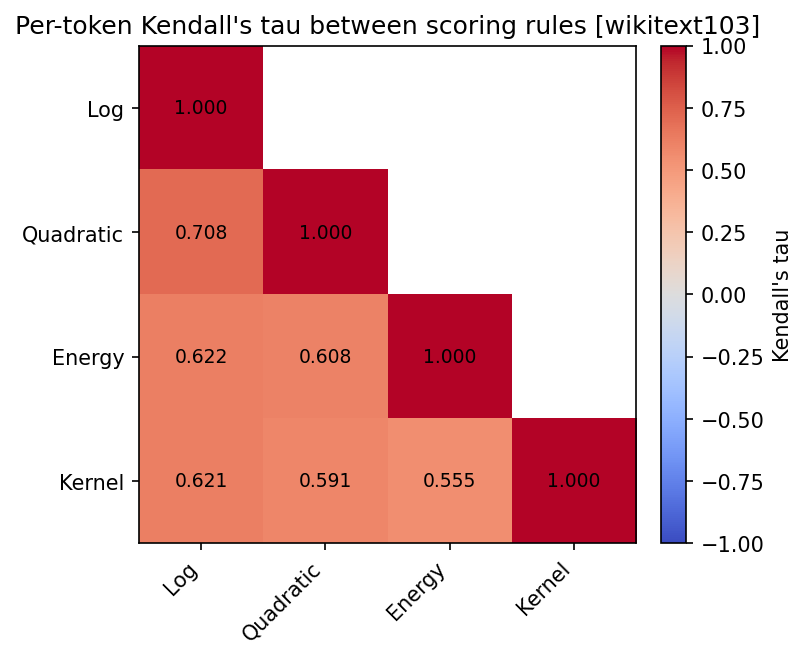
\includegraphics[width=0.42\linewidth]{figures/exp1_kendall_tau_matrix_wikitext103.png}\hspace{0.015\linewidth}
  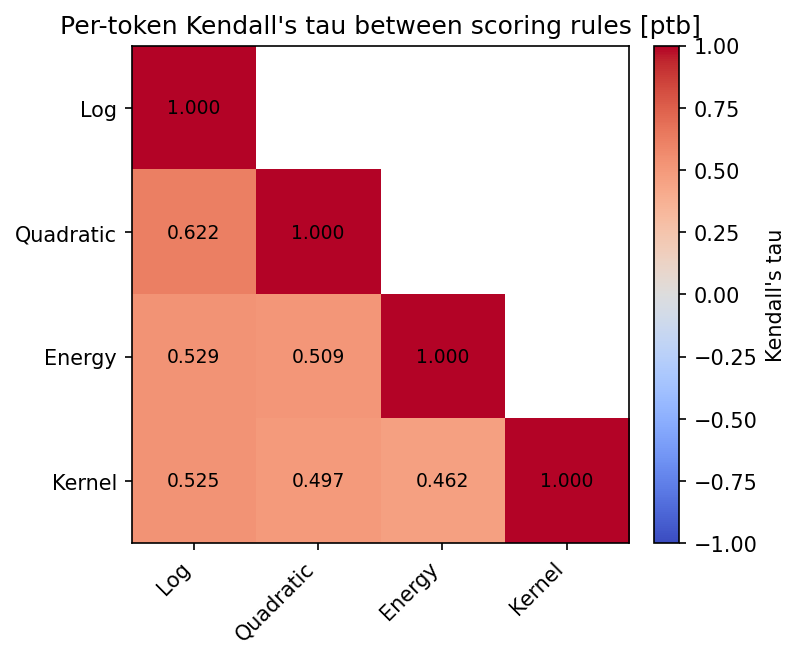
\includegraphics[width=0.42\linewidth]{figures/exp1_kendall_tau_matrix_ptb.png}
  \caption{Experiment 1: token-level Kendall's $\tau$ (defined in
  Appendix~\ref{app:tau}) between per-token scores under the four rules, pooled across
  models. Left: WikiText-103; right: PTB. All pairs lie well below $\tau = 1$.}
  \label{fig:exp1tau}
\end{figure}

By
Equation~\eqref{eq:bregman}, each column of Table~\ref{tab:exp1} estimates the mean
Bregman divergence $d_{\varphi}(\delta_y, P_t)$ between the realized outcomes and the
models' forecasts under that rule's generator. The disagreement between columns is
therefore a statement about geometry: OPT-125M's forecasts are farther from the data
distribution than GPT-2-Medium's when distance is measured by KL divergence, squared
Euclidean distance, or MMD, yet closer when measured by the energy distance taken in each
model's own embedding space. The representation theorem does not merely permit such
reversals; it implies they must occur whenever two models' error structures differ along
directions that two generators curve differently, and
Sections~\ref{sec:exp2}--\ref{sec:exp5} identify those directions. Consistent with this
reading, the rules also disagree pervasively at the level of individual tokens: pairwise
Kendall's $\tau$ between per-token scores lies between $0.46$ and $0.71$ across rule
pairs and corpora (Figure~\ref{fig:exp1tau}).

\section{Experiment 2: tail behavior across token-frequency strata}
\label{sec:exp2}

Scored positions are stratified by the unigram-frequency decile of the target token
(decile 0 containing the most frequent tokens). Figure~\ref{fig:exp2} presents the
resulting penalty profiles. Averaged across models on WikiText-103, the mean log-score
increases by a factor of $2.05$ between decile 0 and decile 8, against $1.22$ for the
quadratic score, $1.58$ for the energy score, and $1.71$ for the kernel score
(corpus-level values in Appendix~\ref{app:amp}).

\begin{figure}[t]
  \centering
  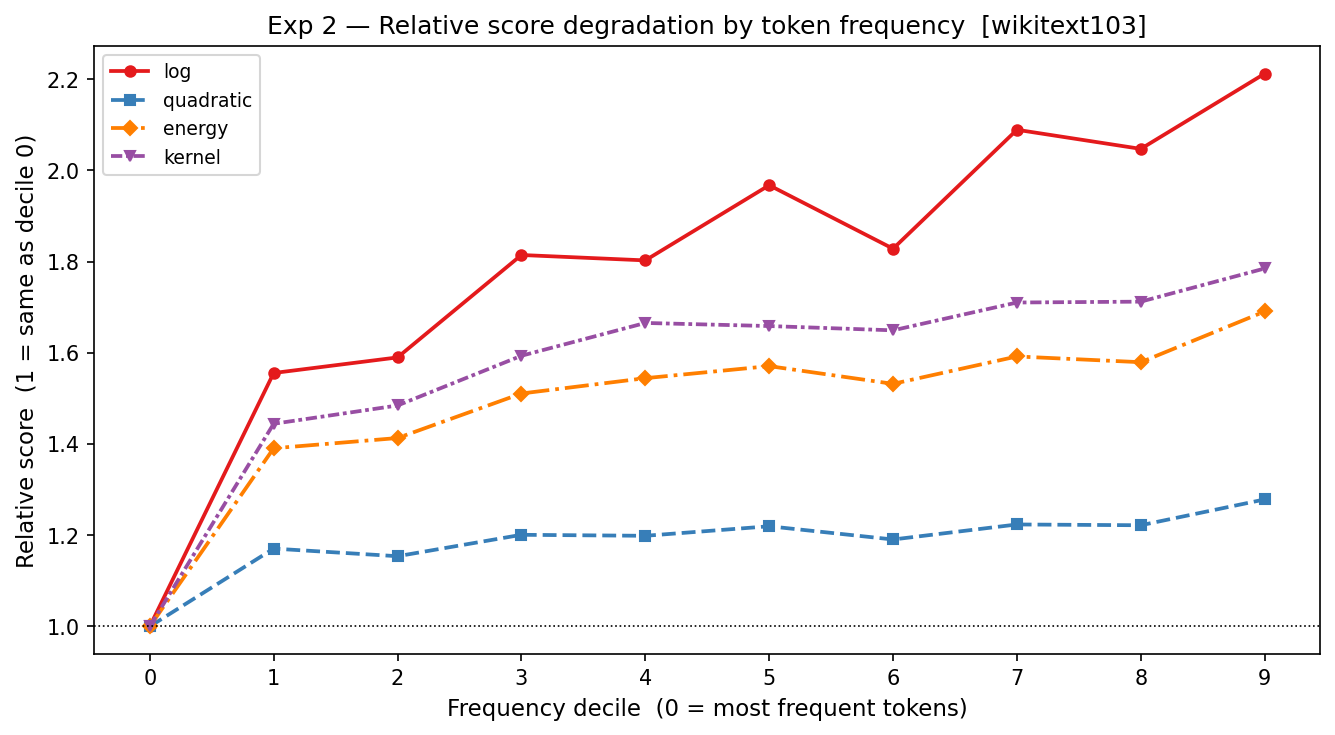
\includegraphics[width=0.49\linewidth]{figures/exp2_wikitext103.png}\hspace{0.01\linewidth}
  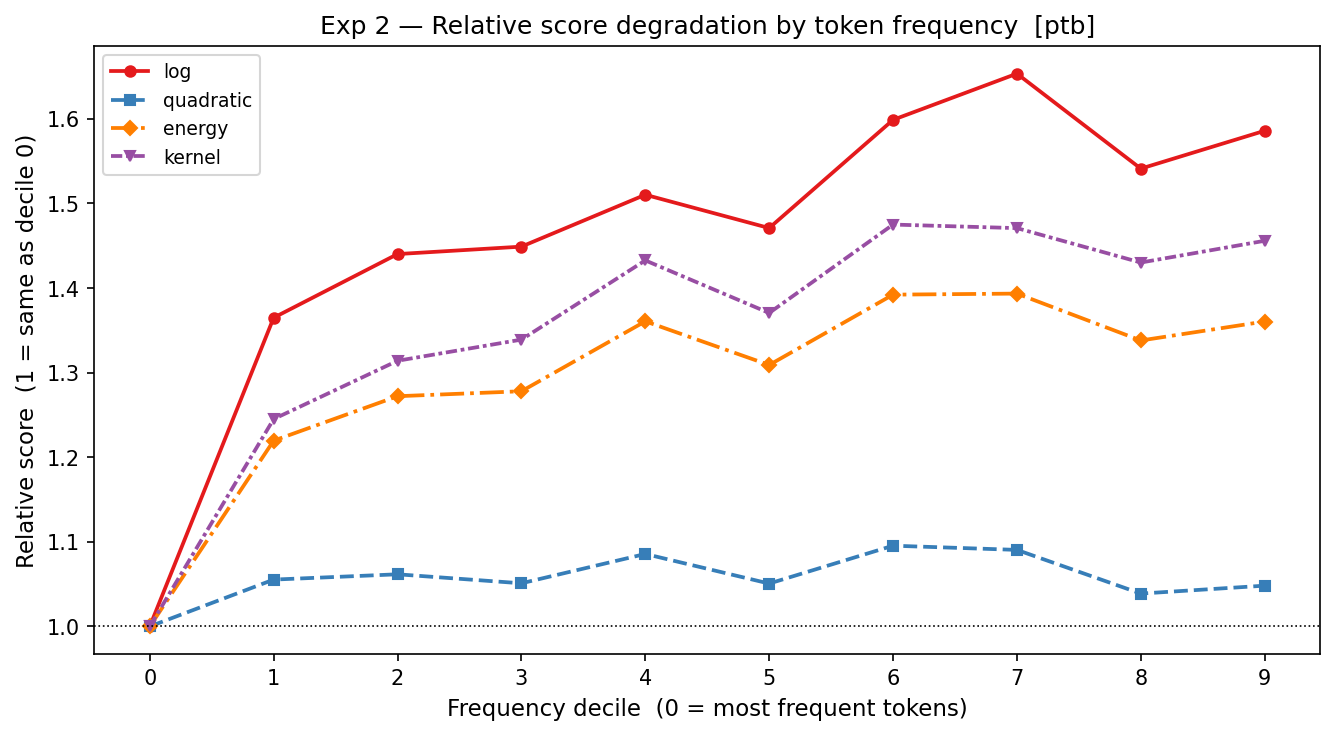
\includegraphics[width=0.49\linewidth]{figures/exp2_ptb.png}
  \caption{Experiment 2: mean score by unigram-frequency decile of the target token
  (left: WikiText-103; right: PTB). The qualitative pattern replicates across corpora.}
  \label{fig:exp2}
\end{figure}

The ordering of these
amplification factors is determined by the boundary behavior of the generators in
Table~\ref{tab:generators}. For the log-score, $d_\varphi(\delta_y, P) = -\log p_y$, and
the curvature $1/p_v$ of the negative-entropy generator diverges as $p_y \to 0$; since
rare targets are precisely those to which models assign small probability, an unbounded
penalty at the simplex boundary is a structural property of KL geometry, not an
empirical accident. The quadratic generator's constant Hessian bounds its divergence by
$2$, and the observed near-flat profile ($1.22\times$) realizes that bound's
consequence. The energy and kernel scores occupy an intermediate position because their
generators penalize rare-token errors through embedding distance rather than through
$p_y$: the penalty grows only insofar as the predictive mass sits far from the target in
feature space. The empirical ordering
$\text{quadratic} < \text{energy} < \text{kernel} < \text{log}$ of tail amplification is
thus exactly the ordering of boundary curvatures of the four generators, as the
representation theorem requires.

\section{Experiment 3: score behavior under predictive uncertainty}
\label{sec:exp3}

\begin{figure}[t]
  \centering
  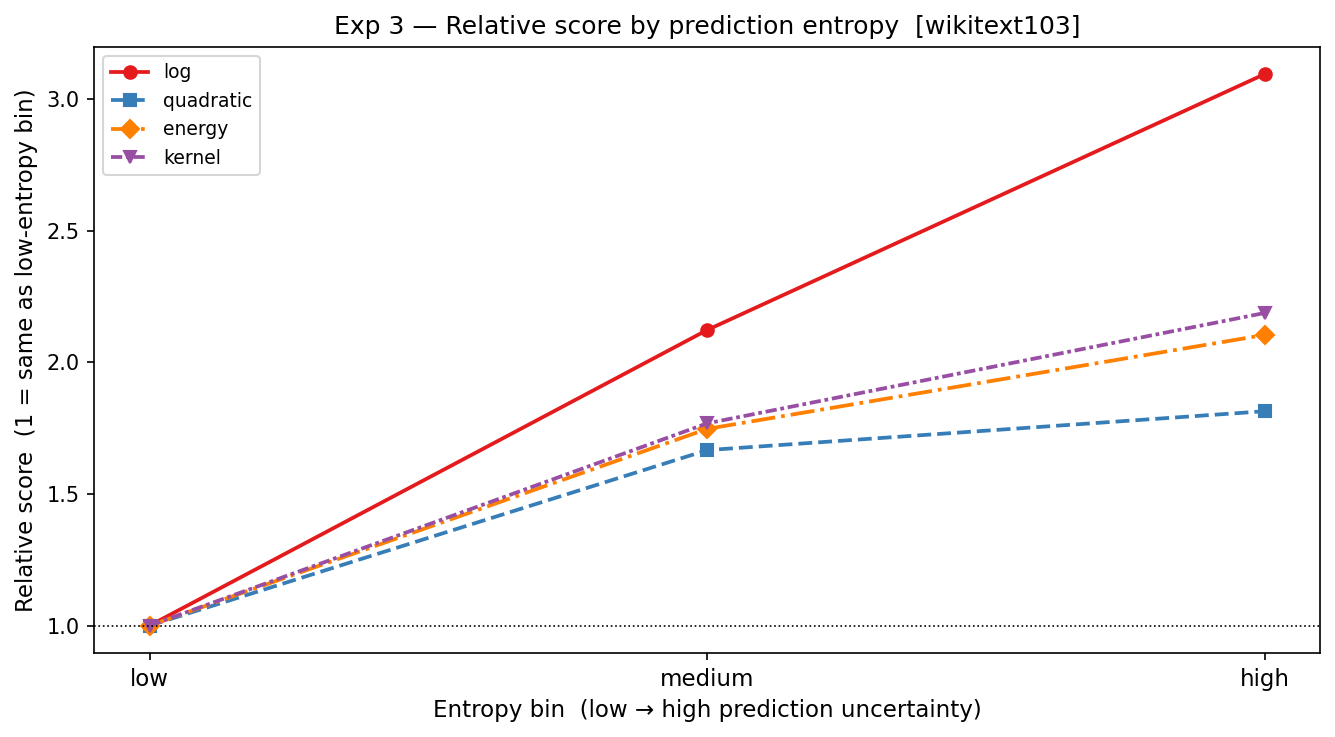
\includegraphics[width=0.49\linewidth]{figures/exp3_wikitext103.png}\hspace{0.01\linewidth}
  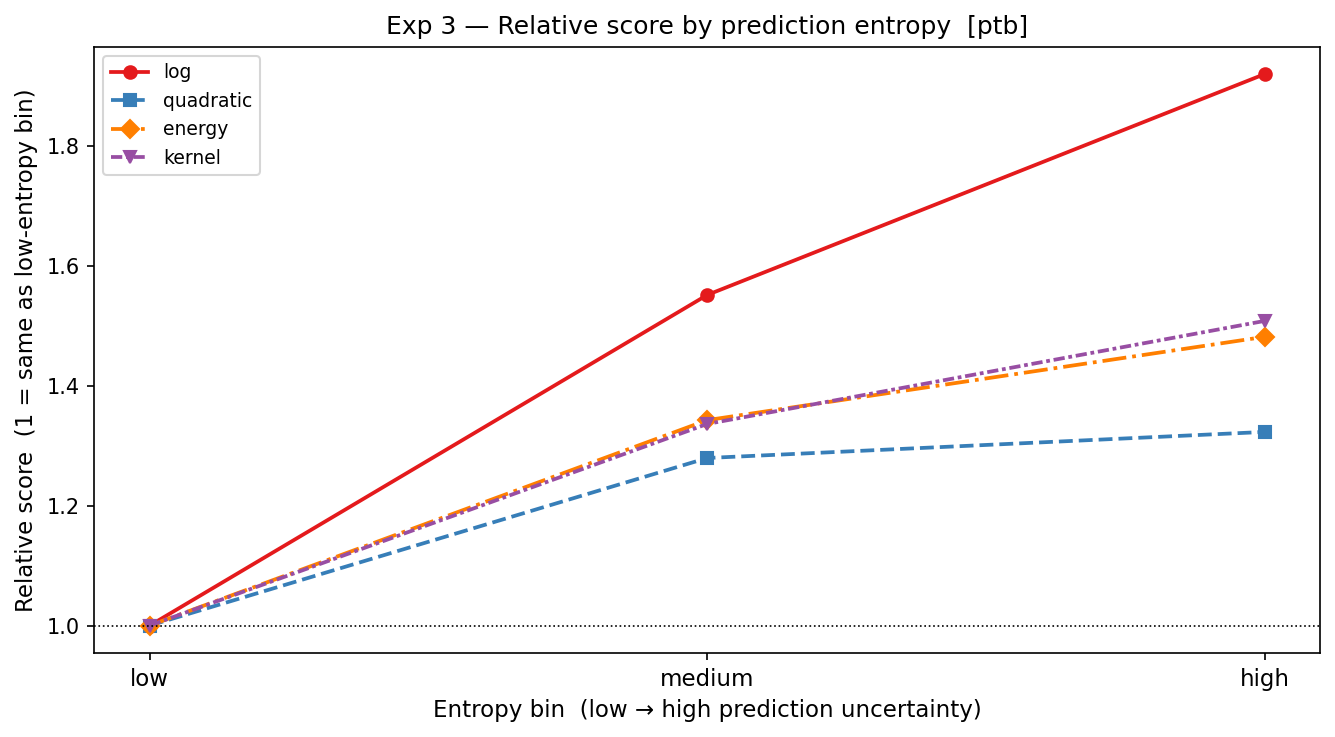
\includegraphics[width=0.49\linewidth]{figures/exp3_ptb.png}
  \caption{Experiment 3: mean score by predictive-entropy tertile (left: WikiText-103;
  right: PTB). The qualitative pattern replicates across corpora.}
  \label{fig:exp3}
\end{figure}

Scored positions are next stratified into per-corpus tertiles of predictive entropy
$H(P) = -\sum_v p_v \log p_v$ (Figure~\ref{fig:exp3}). From the low to the high
tertile on WikiText-103 the mean log-score increases by a factor of $3.09$, the quadratic
by $1.81$, the energy by $2.10$, and the kernel by $2.19$. The more diagnostic statistic
is the ratio between rules: $\Elog / \Eenergy$ rises from $2.58$ in the low tertile to
$3.79$ in the high tertile, an increase of $47\%$ ($29\%$ on PTB;
Appendix~\ref{app:entropy}).

The widening ratio is
a direct manifestation of locality. For the log-score,
$d_{\mathrm{KL}}(\delta_y, P) = -\log p_y$ depends on the forecast only through the mass
assigned to the realized token; a high-entropy forecast necessarily assigns smaller
$p_y$ and is penalized for the diffuseness itself, irrespective of where the remaining
mass is placed. The energy divergence, by contrast, evaluates the full configuration of
the forecast in embedding space: a diffuse $P$ whose mass remains in the vicinity of
$e(y)$ can stand at a small energy distance from $\delta_y$ even while $-\log p_y$ is
large. The monotone growth of the $\Elog/\Eenergy$ ratio across tertiles on both corpora
is the empirical signature of these two response rates; the bounded, similarity-blind
quadratic generator again sits between the extremes, completing the pattern the
curvatures predict.

\section{Experiment 4: statistical robustness of the ranking disagreement}
\label{sec:exp4}

To assess whether the disagreement of Section~\ref{sec:exp1} could be a sampling
artifact, we apply a nonparametric bootstrap over token positions: for each
(model, corpus) cell the 20{,}000 cached per-token scores are resampled with replacement
$B = 1{,}000$ times, and all rule means and induced rankings are recomputed on each
replicate.

\begin{figure}[t]
  \centering
  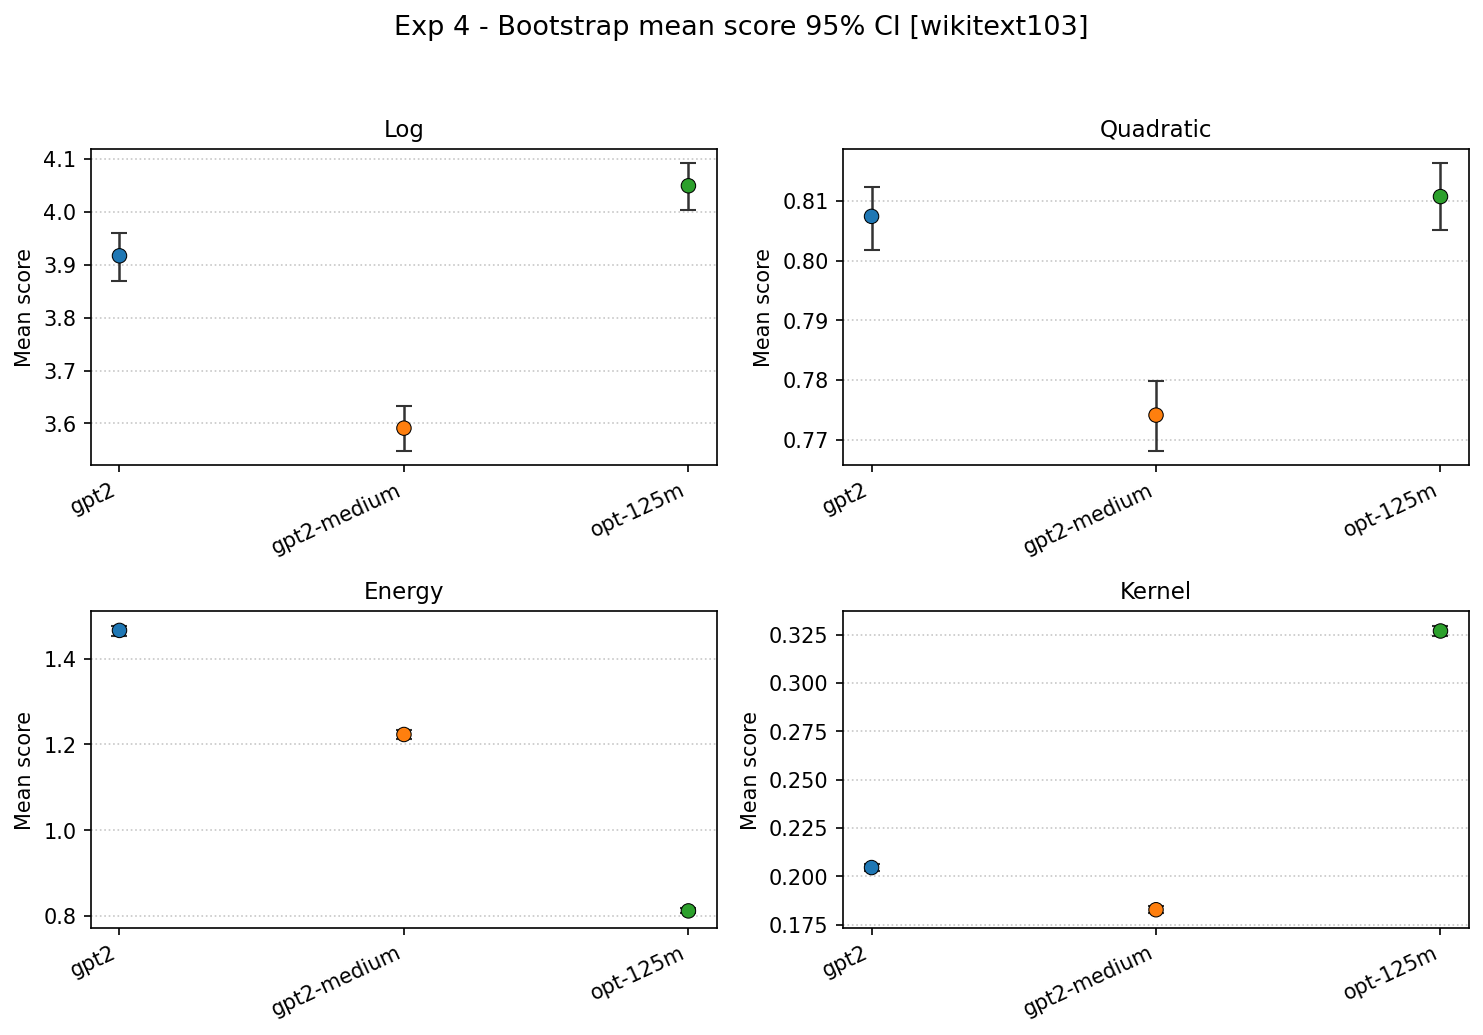
\includegraphics[width=0.49\linewidth]{figures/exp4_score_ci_wikitext103.png}\hspace{0.01\linewidth}
  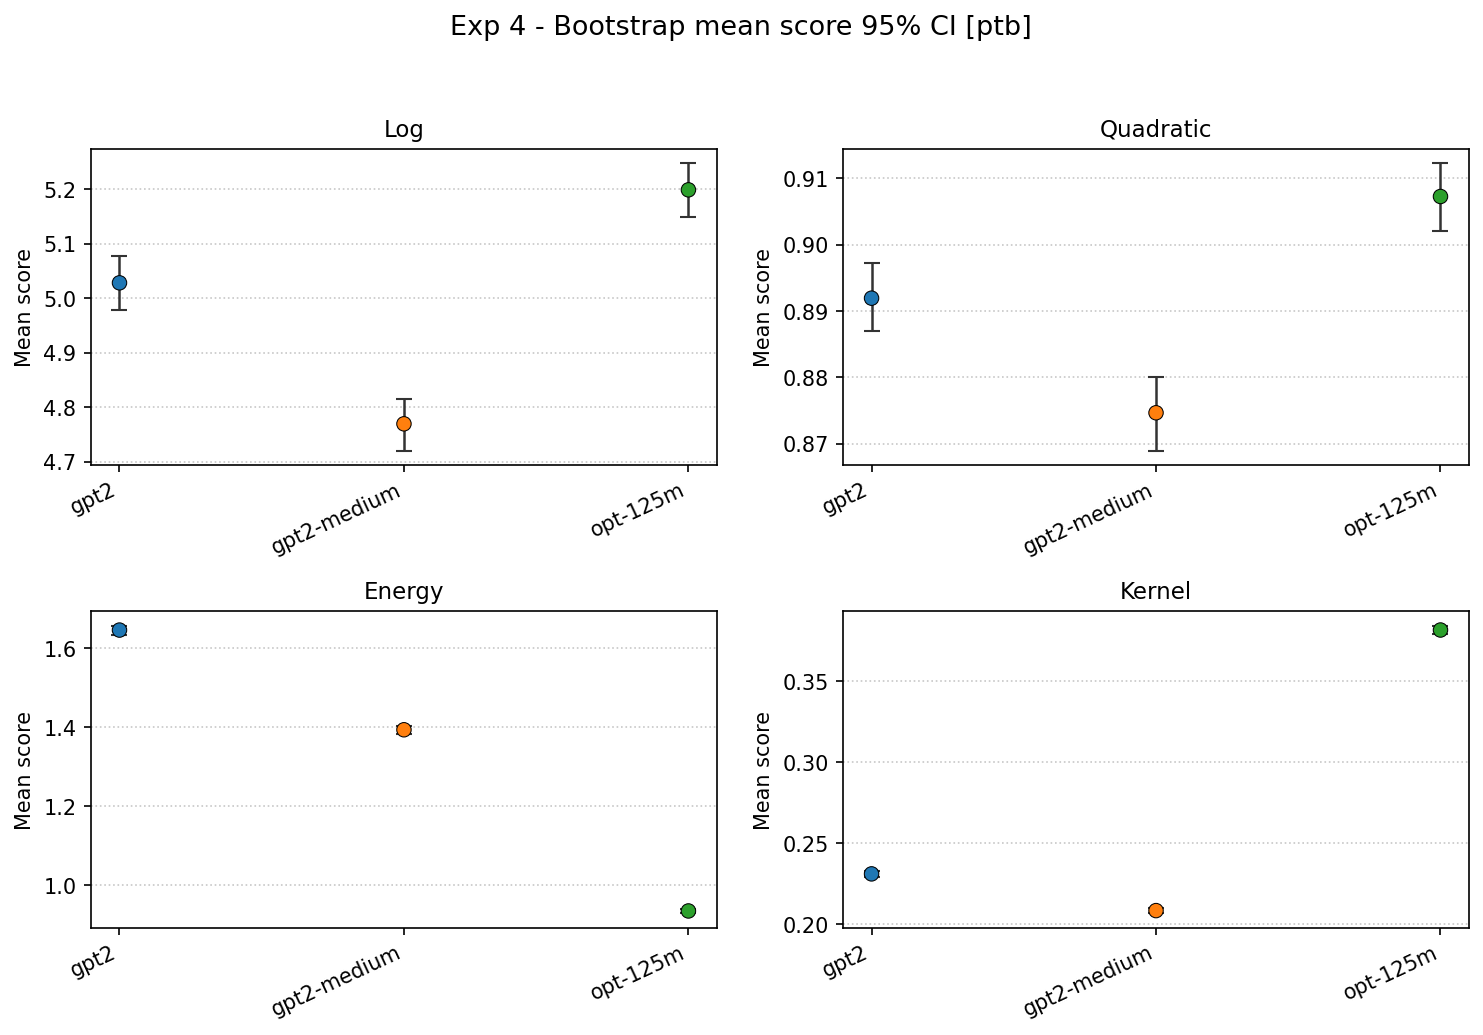
\includegraphics[width=0.49\linewidth]{figures/exp4_score_ci_ptb.png}
  \caption{Experiment 4: bootstrap means and 95\% percentile intervals ($B = 1{,}000$)
  for every (model, rule) cell. Left: WikiText-103; right: PTB. Full tables appear in
  Appendix~\ref{app:boot}.}
  \label{fig:exp4}
\end{figure}

Three results emerge (Figure~\ref{fig:exp4}; Appendix~\ref{app:boot}). First, the 95\%
percentile intervals around all twelve cell means of Table~\ref{tab:exp1} are narrow
relative to the gaps between models, so no pairwise comparison is ambiguous. Second, the
joint event ``OPT-125M is ranked first by the energy score and last by the log-score''
obtains in $100\%$ of replicates on both corpora. Third, the energy ranking agrees with
the log-score ranking in $0\%$ of replicates, the kernel in $100\%$ (quadratic: $80\%$
on WikiText-103, $100\%$ on PTB).

Strict properness
guarantees that each empirical rule mean is a consistent estimator of the corresponding
expected Bregman divergence; the bootstrap addresses the remaining question of whether
the \emph{orderings} of those divergences are estimated stably at $n = 20{,}000$. The
answer is affirmative: the divergence orderings induced by the four generators are
statistically separated, so the cross-rule disagreement of Experiment 1 reflects a
reproducible property of the models' predictive distributions under the four geometries
rather than noise. The bootstrap thereby licenses the mechanistic question taken up in
Experiment 5---\emph{which} structural property of the distributions the energy geometry
is registering.

\section{Experiment 5: an embedding-space account of the energy ranking}
\label{sec:exp5}

The energy divergence between a forecast and a point mass measures, by construction, how
far the forecast's probability mass lies from the realized token in embedding space. Its
first-moment summary is the \emph{predictive barycenter}
$c = \mathbb{E}_{X \sim P}[e(X)] = P^{\top} E$: by Jensen's inequality the leading term
of Equation~\eqref{eq:energy} satisfies
$\mathbb{E}\lVert e(X) - e(y)\rVert \ge \lVert c - e(y) \rVert$, so the barycenter
distance $\lVert c - e(y)\rVert$ is a lower envelope of the energy penalty and a natural
per-event diagnostic of what the energy score responds to. If the Bregman account of
Experiment 1 is correct, the model ranked best by the energy rule should be the model
whose barycenters lie closest to the realized tokens---most consequentially on
\emph{misprediction events} ($64$--$78\%$ of positions depending on cell), where the log
and energy geometries render their most divergent verdicts.

\begin{figure}[t]
  \centering
  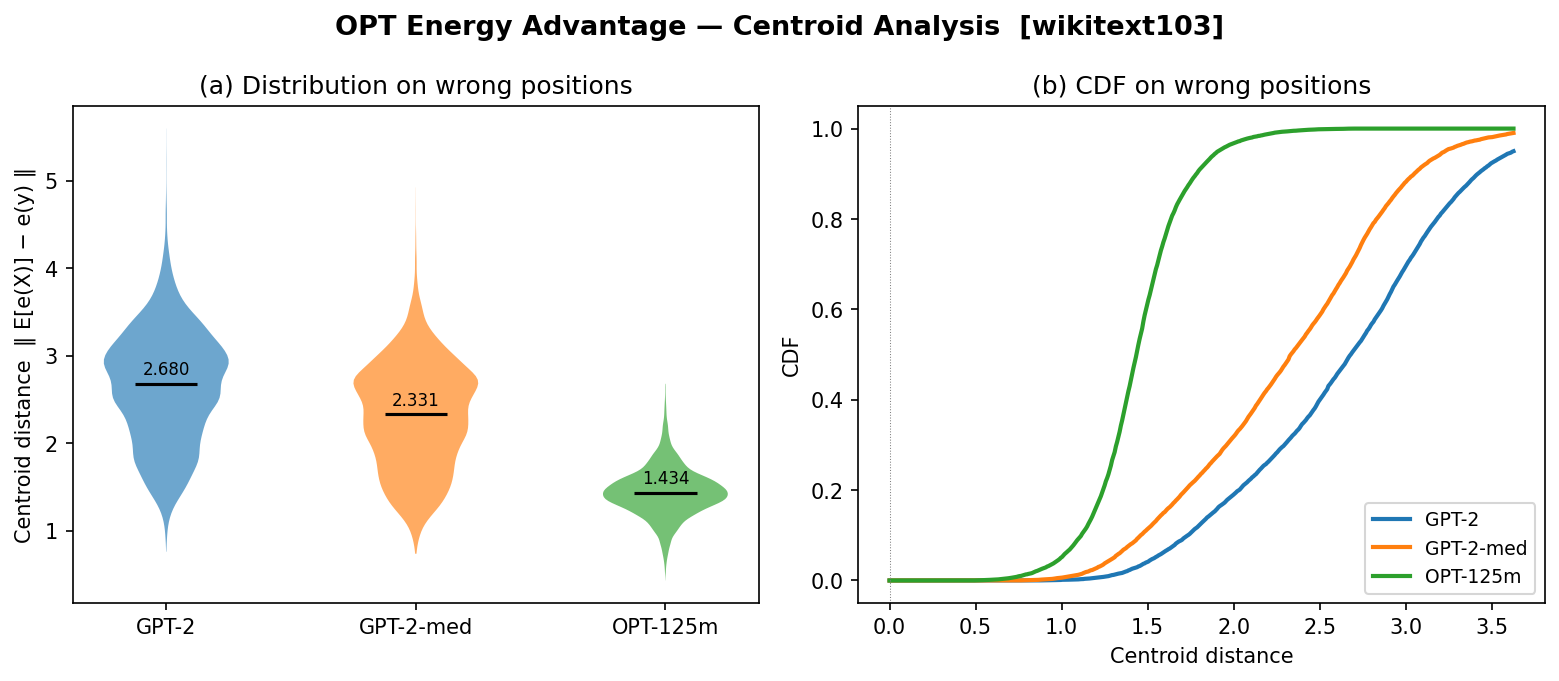
\includegraphics[width=0.78\linewidth]{figures/exp5_wikitext103.png}\\[2pt]
  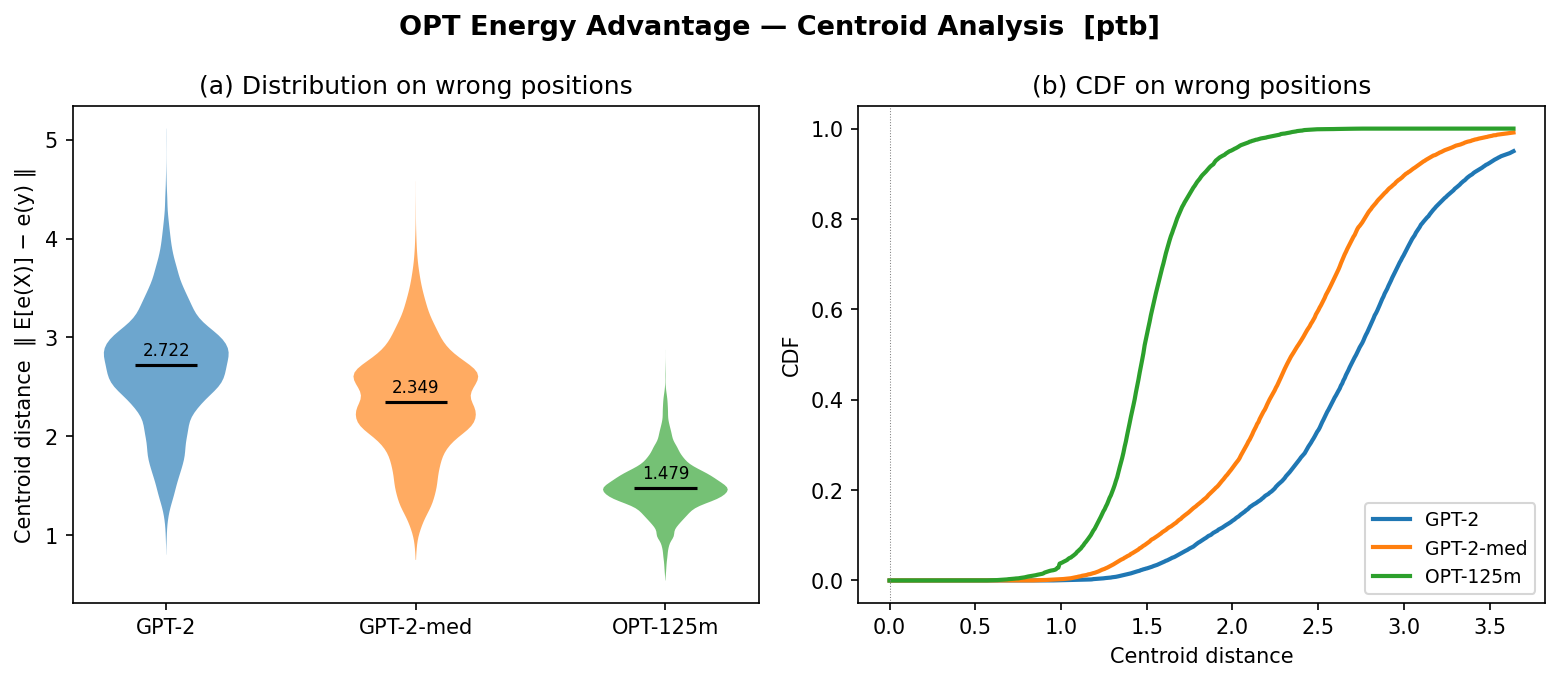
\includegraphics[width=0.78\linewidth]{figures/exp5_ptb.png}
  \caption{Experiment 5: barycenter-to-target distance
  $\lVert \mathbb{E}_P[e(X)] - e(y)\rVert$ on misprediction events (top row:
  WikiText-103; bottom row: PTB). Within each row: distribution by model (black bar
  denotes the median) and empirical CDF. On both corpora the ordering of the three
  distributions reproduces the energy-score ranking of Table~\ref{tab:exp1}.}
  \label{fig:exp5}
\end{figure}

Figure~\ref{fig:exp5} confirms the prediction. On WikiText-103 misprediction events the
mean barycenter distance is $1.44$ for OPT-125M, $2.30$ for GPT-2-Medium, and $2.63$ for
GPT-2 (PTB: $1.49$, $2.34$, $2.69$)---exactly the energy-score ordering of
Table~\ref{tab:exp1}, on both corpora; the same ordering holds for the distance from the
modal (top-1) token to the target (Appendix~\ref{app:exp5}).

Experiment 5 closes
the explanatory chain opened by Experiment 1. The energy generator's divergence is small
exactly when the forecast's mass configuration sits near the target in feature space;
the barycenter distance isolates that quantity event by event, and the model ordering it
produces is the energy ordering---computed without reference to the score itself. The
log-score, whose divergence $-\log p_y$ is invariant to the embedding locations of the
off-target mass, has no access to this structure and accordingly ranks the same events
differently. Each rule is thus observed to be ``satisfied'' in precisely the sense the
representation theorem specifies: its empirical verdict tracks its own generator's
divergence, evaluated on the structural feature of the forecasts that the generator
curves against. The corresponding scope restriction is taken up in
Section~\ref{sec:discussion}.

\section{Discussion}
\label{sec:discussion}

\paragraph{Rankings are rule-relative, as the representation theorem requires.}
Reporting a single rule reports a single geometry, and the choice of that geometry is
substantive, not conventional: the tail and entropy sensitivities of Experiments~2--3
are properties of the log-score's generator, not of the models. Neither is a defect, but
evaluations that care about calibration on common tokens, or that do not wish to
penalize acknowledged ambiguity, will reach materially different conclusions from a
bounded rule obtained at negligible additional computational cost.

\paragraph{What embedding-space scoring contributes.} The energy and kernel scores are
the only rules in the suite whose generators are defined through a metric on tokens, and
they extend evaluation in three directions: they award partial credit for semantically
structured errors, which the log-score penalizes identically to arbitrary ones; they
retain discriminative range where the log-score is dominated by position difficulty
(rare targets, high-entropy contexts; Experiments 2--3); and the kernel bandwidth
supplies a resolution parameter, with small $\sigma$ approaching exact-match evaluation
and large $\sigma$ the energy rule's diffuse assessment, so one strictly proper family
spans several semantic scales.

\paragraph{Scope of cross-model embedding comparisons.} The representation theorem also
delimits what embedding-based comparisons can claim: when each model supplies its own
embedding matrix the resulting divergences are defined over different metric spaces, and
cross-model differences mix properties of the forecasts with properties of the
representations. Within-model comparisons hold the geometry fixed and are free of this
caveat; cross-model comparisons are sharpest when the feature map is fixed by design,
e.g.\ a common reference embedding space.

\paragraph{Future directions.} Two extensions appear most promising. The first is the
systematic study of reference embedding spaces for cross-model comparison, as noted
above. The second moves the energy score from evaluation to estimation. In the
regression setting, \citet{shen2024} introduce \emph{engression}, in which a generative
model of $Y \mid X$ is fitted by minimizing the expected energy score; strict properness
guarantees that the population minimizer is the true conditional distribution. Next-token
prediction is formally the same problem, suggesting that language models could be fitted
or fine-tuned against the energy score in embedding space, in direct analogy to
engression---minimizing the energy divergence rather than the KL divergence of maximum
likelihood, with gradients that do not diverge on rare targets and that reward
semantically structured uncertainty (Experiments 2--3). Whether this improves
calibration at scale is an open question this framework is positioned to test.

\paragraph{Limitations.} The study covers three sub-500M-parameter models and two
English corpora; the geometric mechanisms documented here are properties of the scoring
rules and should transfer, but the specific rankings need not. The energy and kernel
scores are Monte Carlo estimates ($m = 200$) with negligible standard errors
(Appendix~\ref{app:boot}). A frequency-ranked CRPS variant was computed but excluded, as
the total order it requires is arbitrary for tokens.

\section{Conclusion}

Perplexity evaluates a high-dimensional predictive object through a single Bregman
geometry. Scoring identical predictions under four strictly proper rules shows that the
geometries mostly concur, that their one persistent disagreement is statistically
robust, and that every observed pattern is the one the Savage--Bregman representation
requires. Evaluations should accordingly report at least one bounded rule and, where
token similarity matters, one embedding-aware rule alongside perplexity. Proper scoring
rules disagree only where models genuinely differ; reading those disagreements through
their generators converts a nuisance of evaluation into an instrument of analysis.

\begin{thebibliography}{9}
\footnotesize
\setlength{\bibsep}{3pt}

\bibitem[Gneiting and Raftery(2007)]{gneiting2007}
Gneiting, T. and Raftery, A.~E. (2007).
\newblock Strictly proper scoring rules, prediction, and estimation.
\newblock \emph{Journal of the American Statistical Association},
102(477):359--378.

\bibitem[Gretton et~al.(2012)]{gretton2012}
Gretton, A., Borgwardt, K.~M., Rasch, M.~J., Sch\"olkopf, B., and Smola, A. (2012).
\newblock A kernel two-sample test.
\newblock \emph{Journal of Machine Learning Research}, 13:723--773.

\bibitem[Jelinek et~al.(1977)]{jelinek1977}
Jelinek, F., Mercer, R.~L., Bahl, L.~R., and Baker, J.~K. (1977).
\newblock Perplexity---a measure of the difficulty of speech recognition tasks.
\newblock \emph{Journal of the Acoustical Society of America}, 62(S1):S63.

\bibitem[Shen and Meinshausen(2024)]{shen2024}
Shen, X. and Meinshausen, N. (2024).
\newblock Engression: Extrapolation through the lens of distributional regression.
\newblock \emph{Journal of the Royal Statistical Society, Series B}, 86(5):1361--1389.

\bibitem[Radford et~al.(2019)]{radford2019}
Radford, A., Wu, J., Child, R., Luan, D., Amodei, D., and Sutskever, I. (2019).
\newblock Language models are unsupervised multitask learners.
\newblock OpenAI Technical Report.

\bibitem[Steinwart and Ziegel(2021)]{steinwart2021}
Steinwart, I. and Ziegel, J.~F. (2021).
\newblock Strictly proper kernel scores and characteristic kernels on compact spaces.
\newblock \emph{Applied and Computational Harmonic Analysis}, 51:510--542.

\bibitem[Sz\'ekely and Rizzo(2013)]{szekely2013}
Sz\'ekely, G.~J. and Rizzo, M.~L. (2013).
\newblock Energy statistics: A class of statistics based on distances.
\newblock \emph{Journal of Statistical Planning and Inference}, 143(8):1249--1272.

\bibitem[Zhang et~al.(2022)]{zhang2022}
Zhang, S., Roller, S., Goyal, N., et~al. (2022).
\newblock {OPT}: Open pre-trained transformer language models.
\newblock arXiv:2205.01068.

\end{thebibliography}

\appendix
\raggedbottom
\setlength{\intextsep}{6pt}
\renewcommand{\arraystretch}{0.92}

\section{Implementation details}
\label{app:impl}

\paragraph{Pipeline.} Each (model, corpus) cell is processed in a single autoregressive
pass: documents are tokenized (maximum length 512, special tokens added), logits are
computed for positions $1,\dots,T-1$, and all rules are evaluated on the softmax of the
same logits, so every rule scores the identical prediction events. Scoring terminates
once 20{,}000 positions are accumulated per cell. All analyses are deterministic given
the cached per-token arrays; analysis scripts fix the random seed at 591.

\paragraph{Monte Carlo estimators.} For the energy score we use the paired-sample form:
with $X_1,\dots,X_m$ and $X'_1,\dots,X'_m$ drawn independently from $P$ ($m=200$),
\[
  \widehat{S}_{\mathrm{E}} \;=\; \frac{1}{m}\sum_{i=1}^m \lVert e(X_i) - e(y)\rVert
  \;-\; \frac{1}{2m}\sum_{i=1}^m \lVert e(X_i) - e(X'_i)\rVert ,
\]
which is unbiased for Equation~\eqref{eq:energy}; the kernel score uses the analogous
plug-in for Equation~\eqref{eq:kernel} with $k(e(y),e(y)) = 1$. No $T \times V$
intermediate matrices are materialized, keeping memory $O(Tmd)$.

\paragraph{Bandwidths.} The median heuristic estimates $\sigma_0$ from 20{,}000 random
embedding pairs drawn from a 2{,}000-row subsample of each model's embedding matrix.

\paragraph{Compute.} All experiments run on CPU (Windows 11, no GPU); the full suite
(Experiments 1--5, both corpora, three models) completes in approximately six hours,
dominated by the $3 \times 2 \times 20{,}000$ forward passes. Code, configuration, and
per-token score caches are included in the project repository.

\section{Token-level Kendall's $\tau$ between rules}
\label{app:tau}

\begin{definition}[Kendall's rank correlation coefficient]
Let $(x_1, y_1), \dots, (x_n, y_n)$ be paired observations---here, the scores assigned to
the same $n$ token positions by two scoring rules. A pair of indices $(i,j)$, $i<j$, is
\emph{concordant} if the two rules order the positions identically, i.e.\ if
$(x_i - x_j)(y_i - y_j) > 0$, and \emph{discordant} if
$(x_i - x_j)(y_i - y_j) < 0$. Kendall's coefficient is
\[
  \tau \;=\; \frac{n_c - n_d}{\binom{n}{2}},
\]
where $n_c$ and $n_d$ count concordant and discordant pairs. Thus $\tau = 1$ indicates
that the two rules induce identical orderings of the prediction events, $\tau = -1$
exactly reversed orderings, and $\tau = 0$ orderings that agree no more often than
chance. In the presence of ties we report the standard tie-adjusted variant $\tau_b$,
which replaces $\binom{n}{2}$ by the geometric mean of the numbers of untied pairs in
each variable (as implemented in SciPy). Because $\tau$ depends on the scores only
through their ranks, it is invariant to any monotone transformation of either rule and
is therefore a natural measure of agreement between scoring rules whose numerical scales
are not comparable.
\end{definition}

\begin{table}[H]
  \caption{Pairwise Kendall's $\tau$ between per-token scores, pooled across models
  (10{,}000-position subsample per corpus; all $p < 10^{-6}$).}
  \label{tab:tau}
  \centering
  \small
  \begin{tabular}{lcc}
    \toprule
    Rule pair & WikiText-103 & PTB \\
    \midrule
    Log -- Quadratic    & 0.708 & 0.622 \\
    Log -- Energy       & 0.622 & 0.529 \\
    Log -- Kernel       & 0.621 & 0.526 \\
    Quadratic -- Energy & 0.608 & 0.509 \\
    Quadratic -- Kernel & 0.591 & 0.497 \\
    Energy -- Kernel    & 0.555 & 0.462 \\
    \bottomrule
  \end{tabular}
\end{table}

\section{Bootstrap tables}
\label{app:boot}

\begin{table}[H]
  \caption{Bootstrap ($B = 1{,}000$ resamples of 20{,}000 token positions) standard
  errors and 95\% percentile intervals for every cell of Table~\ref{tab:exp1},
  WikiText-103. All cross-model gaps exceed ten standard errors.}
  \label{tab:bootci}
  \centering
  \small
  \begin{tabular}{llcccc}
    \toprule
    Model & Rule & Mean & SE & CI$_{2.5}$ & CI$_{97.5}$ \\
    \midrule
    GPT-2        & Log       & 3.917 & 0.024 & 3.870 & 3.964 \\
    GPT-2        & Quadratic & 0.807 & 0.003 & 0.801 & 0.813 \\
    GPT-2        & Energy    & 1.466 & 0.006 & 1.453 & 1.477 \\
    GPT-2        & Kernel    & 0.205 & 0.001 & 0.203 & 0.206 \\
    GPT-2-Medium & Log       & 3.591 & 0.024 & 3.545 & 3.638 \\
    GPT-2-Medium & Quadratic & 0.774 & 0.003 & 0.768 & 0.780 \\
    GPT-2-Medium & Energy    & 1.223 & 0.005 & 1.212 & 1.233 \\
    GPT-2-Medium & Kernel    & 0.183 & 0.001 & 0.181 & 0.185 \\
    OPT-125M     & Log       & 4.049 & 0.025 & 4.001 & 4.097 \\
    OPT-125M     & Quadratic & 0.811 & 0.003 & 0.805 & 0.816 \\
    OPT-125M     & Energy    & 0.812 & 0.003 & 0.806 & 0.818 \\
    OPT-125M     & Kernel    & 0.327 & 0.001 & 0.324 & 0.330 \\
    \bottomrule
  \end{tabular}
\end{table}

Event probabilities across replicates (identical on both corpora):
$\Pr[\text{OPT-125M ranked first under energy}] = 1.00$;
$\Pr[\text{OPT-125M ranked last under log}] = 1.00$;
$\Pr[\text{both events jointly}] = 1.00$.
Fraction of replicates whose full three-model ranking matches the log-score ranking:
energy $0.00$, kernel $1.00$, quadratic $0.80$ on WikiText-103;
energy $0.00$, kernel $1.00$, quadratic $1.00$ on PTB.

\section{Experiment 5 summary statistics}
\label{app:exp5}

\begin{table}[H]
  \caption{Barycenter and modal-token distances to the target on misprediction events
  (mean over events; PTB in parentheses). The ordering of either column reproduces the
  energy-score ranking of Table~\ref{tab:exp1} on both corpora.}
  \label{tab:exp5app}
  \centering
  \small
  \begin{tabular}{lccc}
    \toprule
    Model & \% positions mispredicted & Barycenter dist. & Top-1 dist. \\
    \midrule
    GPT-2        & 67.9 (76.9) & 2.63 (2.69) & 3.50 (3.51) \\
    GPT-2-Medium & 64.3 (74.6) & 2.30 (2.34) & 3.03 (3.01) \\
    OPT-125M     & 68.7 (78.2) & 1.44 (1.49) & 2.01 (2.04) \\
    \bottomrule
  \end{tabular}
\end{table}

\section{Experiment 2 amplification factors}
\label{app:amp}

\begin{table}[H]
  \caption{Ratio of mean score at frequency decile 8 (rare) to decile 0 (common),
  averaged across models.}
  \label{tab:amp}
  \centering
  \small
  \begin{tabular}{lcccc}
    \toprule
    Corpus & Log & Quadratic & Energy & Kernel \\
    \midrule
    WikiText-103 & 2.05$\times$ & 1.22$\times$ & 1.58$\times$ & 1.71$\times$ \\
    PTB          & 1.54$\times$ & 1.04$\times$ & 1.34$\times$ & 1.43$\times$ \\
    \bottomrule
  \end{tabular}
\end{table}

\section{Experiment 3 entropy-tertile ratios}
\label{app:entropy}

\begin{table}[H]
  \caption{Mean log-to-energy and log-to-kernel score ratios by predictive-entropy
  tertile, averaged across models.}
  \label{tab:entropy}
  \centering
  \small
  \begin{tabular}{llcc}
    \toprule
    Corpus & Tertile & Log/Energy & Log/Kernel \\
    \midrule
    \multirow{3}{*}{WikiText-103} & low    & 2.58 & 12.9 \\
                                  & medium & 3.13 & 15.5 \\
                                  & high   & 3.79 & 18.2 \\
    \midrule
    \multirow{3}{*}{PTB}          & low    & 3.23 & 15.7 \\
                                  & medium & 3.73 & 18.2 \\
                                  & high   & 4.18 & 20.0 \\
    \bottomrule
  \end{tabular}
\end{table}

\end{document}
